\section{Implementation \& Parameters}\label{sec:parameters}

%\subsection{Interlink optimizations}

%% A Merkle tree is used to hash the interlink data structure
%% into a single hash \cite{KLS}. NIPoPoWs form a chain of various levels
%% which can omit blocks. For each block in the proof,
%% only a single pointer needs to be presented to convince the Verifier. Near
%% genesis, the pointers needed correspond to high levels; near
%% the tip, the pointers to low levels. In the construction of
%% the proof, the highest superchain with at least $m$ blocks is included, and
%% assume it is of level $\mu$. The level $\mu - 1$ superchain is fully
%% included and has an expected number of $2m$ blocks. Since all
%% $\mu$-superblocks are also $(\mu - 1)$-superblocks, they only need to be
%% counted once, for $\mu - 1$. Among the expected $2m$ $(\mu - 1)$-superblocks,
%% the last $m$ will be supported by level $\mu - 2$. As before, since $(\mu -
%% 1)$-superblocks are $(\mu - 2)$-superblocks, in expectation only $m$
%% $(\mu-1)$-superblocks are counted. The argument continues inductively, until
%% $2m$ $0$-blocks are included in expectation immediately before the $\chi$
%% suffix. This gives an estimation on the proof size: a total of $m
%% (\log(|\chain|) - \log(m))$ blocks in expectation, $m$ at each of the $\mu - 1$
%% levels and $2m$ $0$-blocks.

We now discuss the size of NIPoPoW proofs and evaluate concrete parameters.
Organizing the interlink data structure as a Merkle tree of $\log(|\chain|)$ items, a
proof-of-inclusion is provided in $\log \log(|\chain|)$ space in expectation;
the proof need not include $0$-level pointers, but must include the genesis
block.
Transaction inclusion
\footnote{This additional data is needed if a \emph{soft} or \emph{hard fork} is
to be avoided. For more information about gradual deployment paths, consult the
relevant section in
\ifhasappendix
the appendix.
\else
the full version of this paper.
\fi}
can be proved in the block header in
$\log(|\overline x|)$ using the standard Merkle tree of transactions, where
$\overline x$ denotes the vector of all transactions included in the particular
block.
This makes the proof size require $\log(|\overline x|) +
\log\log(|\chain|)$ hashes per block for a total of
$(2m (\log|\chain| - \log{m}) + m)(\log|\overline x| + \log\log|\chain|)$
hashes. In addition, $m
(\log(|\chain|) - \log(m))$ headers and coinbase transactions are needed. As an
example, given that currently in bitcoin $|\chain| = 464{,}185$ and $|\overline x|
= 2000$, we have $\log(|\chain|) = 18, \log\log(|\chain|) = 5, \log(|\overline
x|) = 11$. For the $k$-suffix, only $k$ headers are needed. We set $k = 6$ and
see that headers are $80$ bytes and hashes $32$ bytes. For the $k$-suffix as
well as the $2m$ $0$-blocks in $\pi$, neither coinbase data nor prev ids are
needed, limiting header size to $48$ bytes. The root and leaves of the pointers
tree can be omitted from coinbase when transmitting the proof. In fact, no block
ids need to be transmitted. From these observations, we estimate our scheme's
proof sizes for various parameterizations of $m$ in Table~\ref{table.size}.

\noindent
\textbf{Concrete parameterization.}
To determine concrete values for security parameter $m$, we focus on a
particular adversarial strategy and analyze its probability of success.
%While other adversarial behaviors may be possible, this attack is
%serves as a baseline for determining specific values for
%$m$.
The attack is an extension of the stochastic processes described in
\cite{bitcoin} and \cite{rosenfeld}.

The experiment works as follows: $m$ is fixed and some adversarial computational
power percentage $q$ of the total network computational power is chosen; $k$ is
chosen based on $q$ according to Nakamoto \cite{bitcoin}. The number of blocks
$y$ during which parallel mining will occur is also fixed. The experiment begins
with the adversary and honest parties sharing a common blockchain which ends in
block $B$. After $B$ is mined, the adversary starts mining in secret and in
parallel with the honest parties on her own private fork on top of $B$. She
ignores the honest chain, so that the two chains remain disjoint after $B$. As
soon as $y$ blocks have been mined in total, the adversary attempts a double
spend via a NIPoPoW
by creating two conflicting transactions which are committed to an honest
block and an adversarial block respectively on top of each current chain.
Finally, the adversary mines $k$ blocks on top of the double spending
transaction within her private chain. After these $k$ blocks have been mined,
she publishes her private chain in an attempt to overcome the honest chain.

\begin{minipage}{\textwidth}
    \begin{minipage}[t]{0.49\textwidth}
      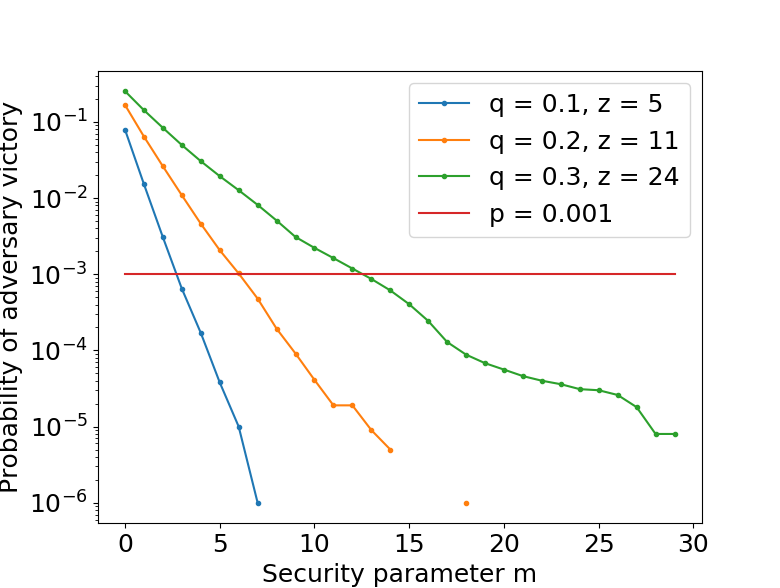
\includegraphics[width=\columnwidth,keepaspectratio]{figures/nipopow-attack-experiment-onecolumn.png}
      \captionof{figure}{\label{fig.nipopow-attack-experiment}
          Mining adversary success rate}
    \end{minipage}
    \hfill
    \begin{minipage}[b]{0.49\textwidth}
      \begin{tabular}{l|l|l|l}
          {\bf m}  & {\bf NIPoPoW size} & {\bf Blocks} & {\bf
          Hashes}\\
          \hline
          $6$   & $70$  kB & $108$ & $1440$  \\
          $15$  & $146$ kB & $231$ & $2925$  \\
          $30$  & $270$ kB & $426$ & $5400$  \\
          $50$  & $412$ kB & $656$ & $8250$ \\
          $100$ & $750$ kB & $1206$ & $15000$ \\
          $127$ & $952$ kB & $1530$ & $19050$ \\
      \end{tabular}
      \captionof{table}{
        \label{table.size}
        NIPoPoWs on Bitcoin
        %and with current values for transaction count, block count,
        %coinbase size and hash output length.
      }
    \end{minipage}
\end{minipage}
\vskip2pt

We measure the probability of success of this attack. We experiment with various
values of $m$ for $y = 100$, indicating $100$ blocks of secret parallel mining.
We make the assumption that honest party communication is perfect and immediate.
We ran $1{,}000{,}000$ Monte Carlo executions\ifanonymous\else\footnote{
Our experiment can be reproduced by running our code available under
an open source MIT license at
\url{https://github.com/dionyziz/popow/tree/master/experiment}}
\fi
of the experiment for each value
of $m$ from $1$ to $30$. We ran the simulation for values of computational power
percentage $q = 0.1$, $q = 0.2$ and $q = 0.3$. The results are plotted in
Figure~\ref{fig.nipopow-attack-experiment}.
Here, $k$ is according to Nakamoto. Based on these data, we conclude that $m = 5$
is sufficient to achieve a $0.001$ probability of failure against an adversary
with $10\%$ mining power. To secure against an adversary with more than $30\%$
mining power, a choice of $m = 15$ is needed.
